\documentclass{standalone}
\usepackage{tikz}
\usepackage{amsmath}
\usetikzlibrary{decorations.pathmorphing, decorations.fractals, shapes}

\begin{document}

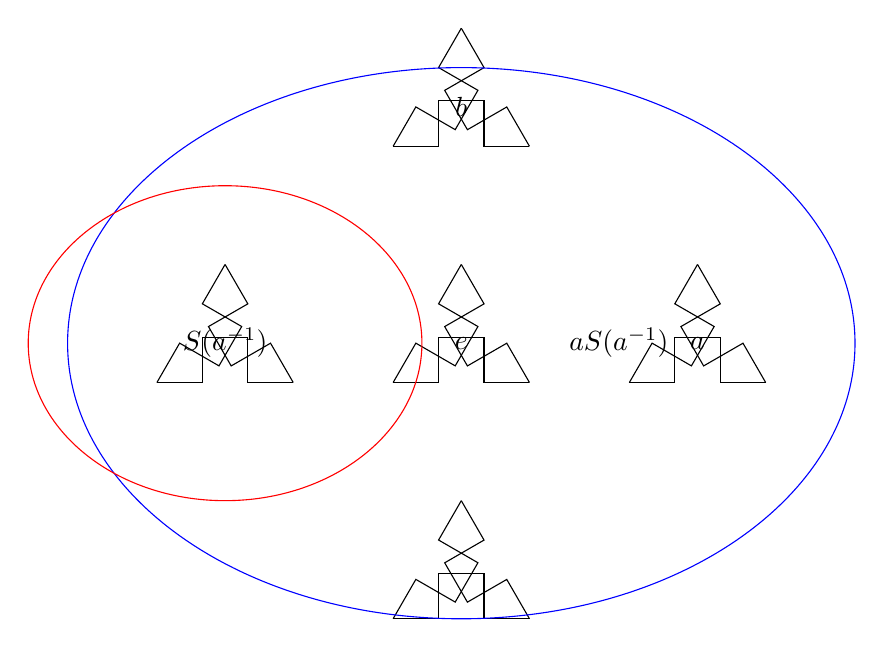
\begin{tikzpicture}

% Fractal definition
\newcommand\fractalscale{0.5}

% Define the Sierpinski triangle fractal
\begin{scope}[shift={(0,0)},scale=\fractalscale]
\foreach \i in {0,1,2} {
	\draw[decorate, decoration={Koch curve type 1}] (90+120*\i:2) -- ({90+120*(\i+1)}:2);
}
\end{scope}

% Define the other fractals and transformations
\begin{scope}[shift={(-3,0)},scale=\fractalscale]
\foreach \i in {0,1,2} {
	\draw[decorate, decoration={Koch curve type 1}] (90+120*\i:2) -- ({90+120*(\i+1)}:2);
}
\end{scope}

\begin{scope}[shift={(3,0)},scale=\fractalscale]
\foreach \i in {0,1,2} {
	\draw[decorate, decoration={Koch curve type 1}] (90+120*\i:2) -- ({90+120*(\i+1)}:2);
}
\end{scope}

\begin{scope}[shift={(0,3)},scale=\fractalscale]
\foreach \i in {0,1,2} {
	\draw[decorate, decoration={Koch curve type 1}] (90+120*\i:2) -- ({90+120*(\i+1)}:2);
}
\end{scope}

\begin{scope}[shift={(0,-3)},scale=\fractalscale]
\foreach \i in {0,1,2} {
	\draw[decorate, decoration={Koch curve type 1}] (90+120*\i:2) -- ({90+120*(\i+1)}:2);
}
\end{scope}

% Draw ellipses and labels
\draw[blue] (0,0) ellipse (5 and 3.5);
\draw[red] (-3,0) ellipse (2.5 and 2);

\node at (-3,0) {$S(a^{-1})$};
\node at (2,0) {$aS(a^{-1})$};
\node at (3,0) {$a$};
\node at (0,3) {$b$};
\node at (0,0) {$e$};

\end{tikzpicture}

\end{document}
